\section{Presentation Logic Layer}

%What pages will be present in your project? briefly indicate how your web site will be organized

WaCar web application is subdivided into two main areas: the admin area and the registered user. The areas are accessible through the login page, where, by inserting a valid combination of email and password, people can access as an admin or a user, depending on the role associated with the email in the database. Below are listed the pages that are going to be developed in WaCar for the users.
\begin{itemize}
    \item Homepage: the initial page presented when connecting to the website. On this page login is not needed and not registered user can see the list or cars and circuit or eventually sign up to the website via the corrispondent page;
    \item Login: the page is used by registered admin/users to login
    \item Sign up: the page is used by new users to sign up to WaCar website;
    \item Car List: the page where the available brand and model of cars are listed;
    \item Circuit List: the page to see the circuits where one can race;
    \item Order List: the page is available only to logged users and allows them to check the order history and manage the them;
    \item Create new order: the page is available to logged users and allows them to create a new order;
    \item List Favorite: the page is available only to logged users and allows them to check their favorite order list;
    \item User Page: the page is available to logged users and allows them to see their informations;\\
\end{itemize}

As it concerns the admin, the following pages have been developed:
\begin{itemize}
    \item Insert Car: in this page are present all the needed fields to create the car: model, brand, description, max speed, horsepower, acceleration, availability, image and type.
    \item Insert Circuit: in this page are present all the needed fields to create the circuit: name, address, description, length, number of corners, lap price, availability, image and type.
    \item Insert Car Type: the page can be used to create a new car type.
    \item Insert Circuit Type: the page can be used to create a new circuit type.
    \item Car-Circuit Suitability: the page can be used to create or delete a matching between a car or a circuit.
    \item Edit Car: the page used to edit an existing car. Here you can for instance modify the description of the car.
    \item Edit Circuit: the page used to edit an existing circuit. Here you can for instance modify the address information of the circuit.
\end{itemize}

\subsection{Sign Up and Login page}

\begin{figure}[h]
  \centering
    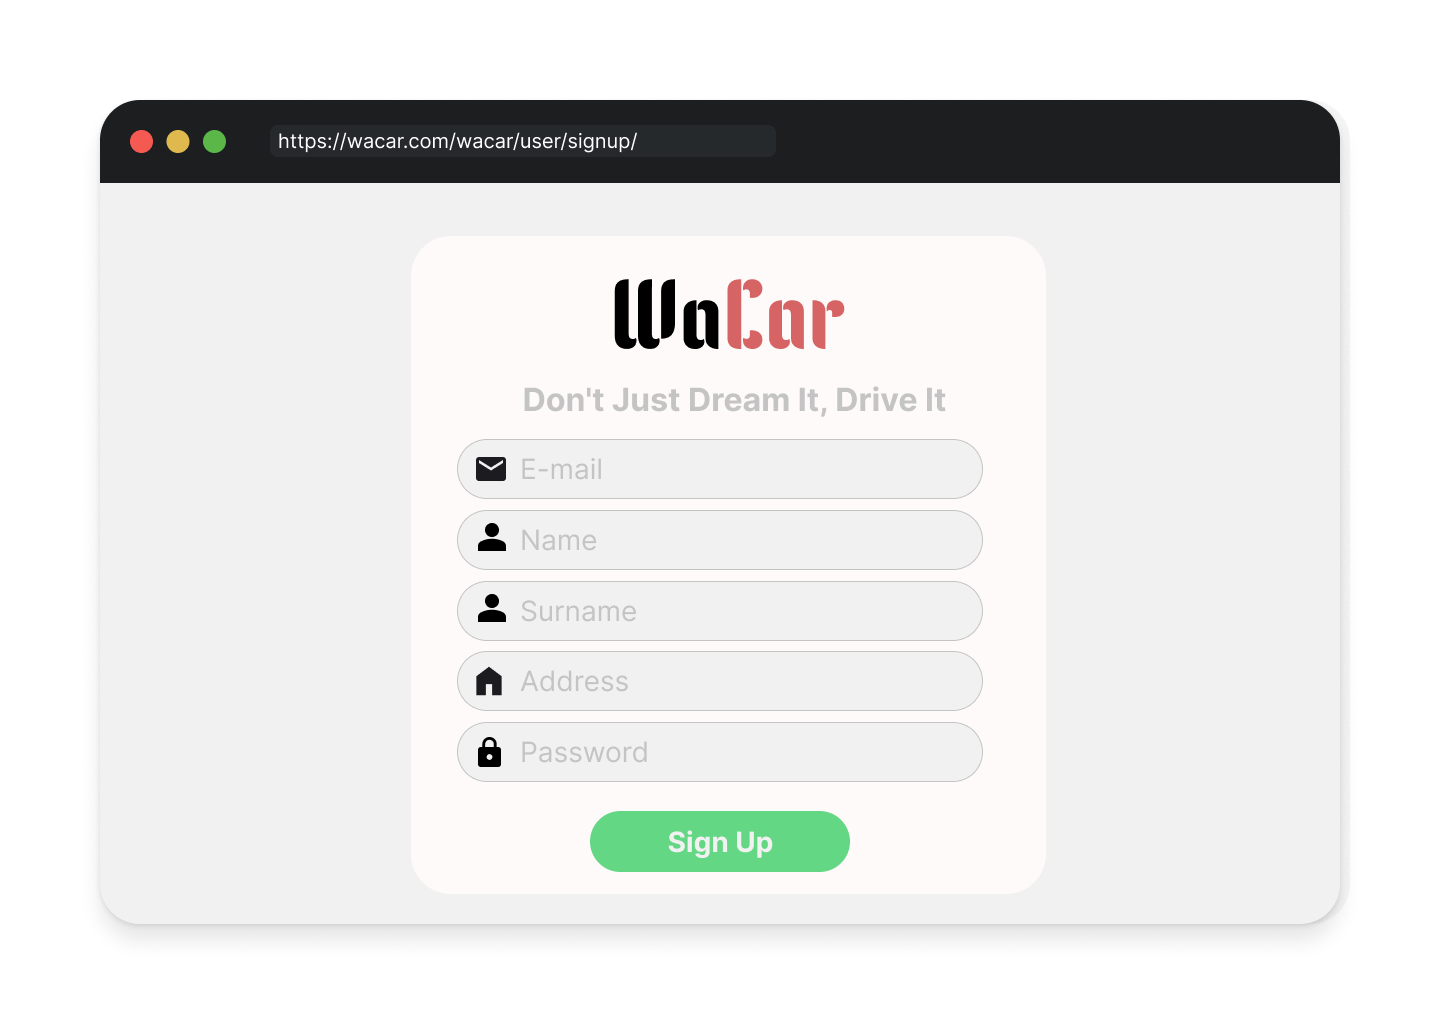
\includegraphics[width=0.6\textwidth]{mockup/SignUp.png}
    \caption{Sign Up page.}
    \label{fig:signup}
\end{figure}

\begin{figure}[h]
    \centering
    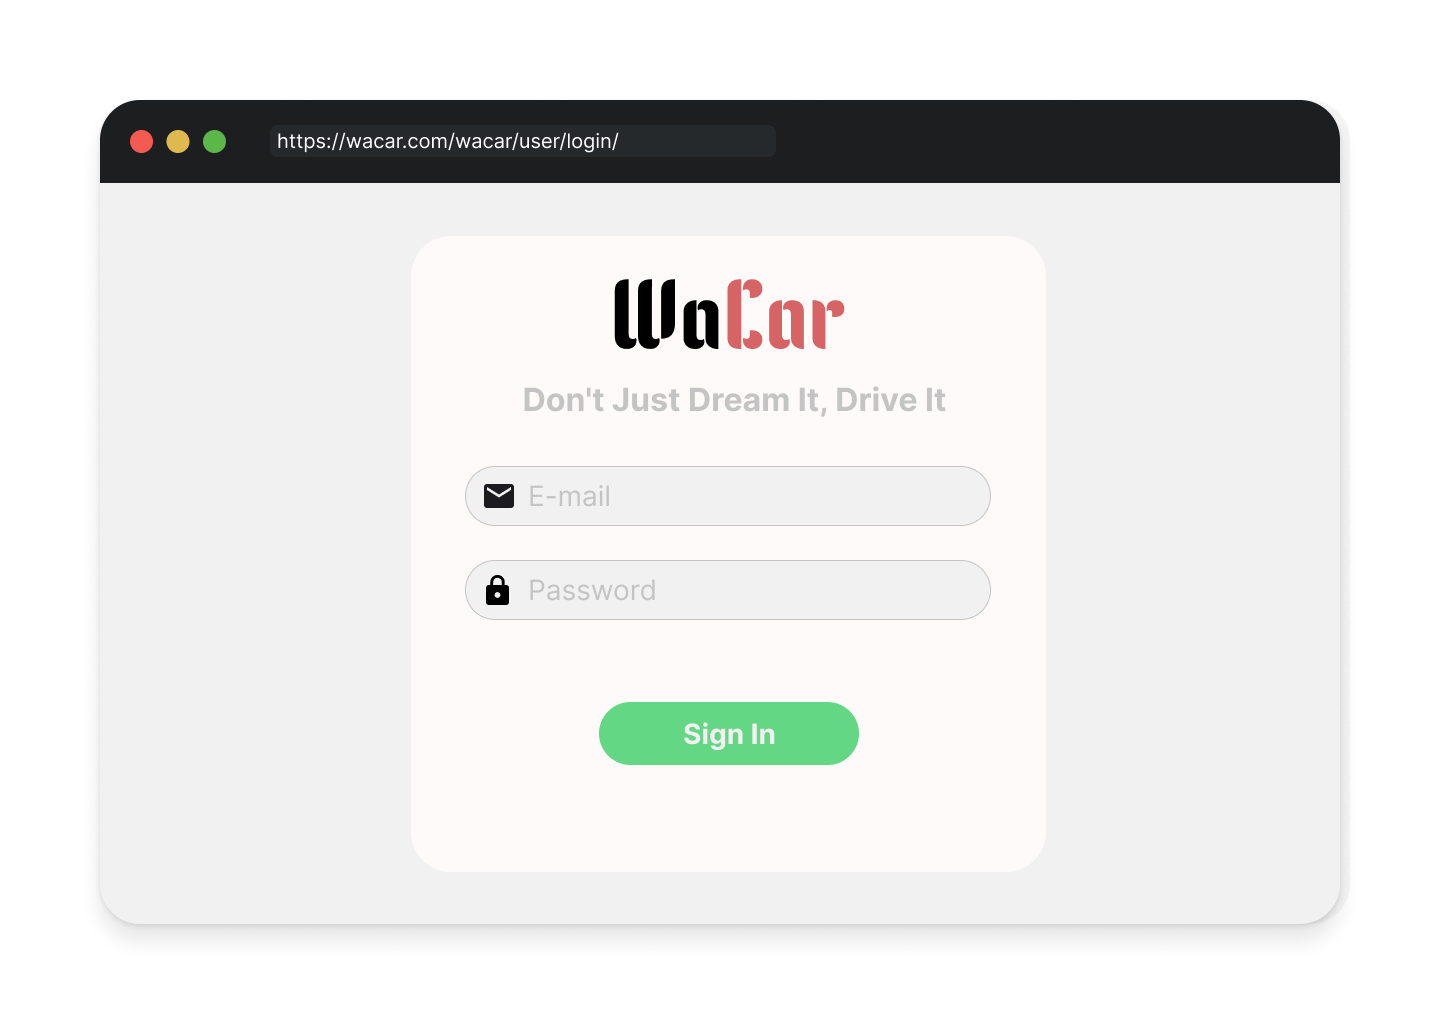
\includegraphics[width=0.6\textwidth]{mockup/Sign in.png}
    \caption{Login page.}
    \label{fig:signin}
\end{figure}

In the \texttt{Sign Up} page, Fig. \ref{fig:signup}, users input their information to create a new account and access to new functionalities. The required information for the registration are email, password, name, surname, and address. The password must meet certain criteria including a minimum of 8 characters, at least one number, and at least one uppercase letter. Upon clicking "Sign up" the user's credentials are added to the database and users are redirected to the homepage. If the provided credentials do not meet the required criteria an error message is displayed to the user. The login process mirrors the sign up process, but only requires the user to input their email and password and upon clicking "Login" a search is conducted in the database, Fig. \ref{fig:signin}. If the provided email exists and the user's password matches the encrypted password stored in the database, the login operation is executed, otherwise the user is informed that email or password are incorrect.

\subsection{Homepage}

\begin{figure}[h]
    \centering
    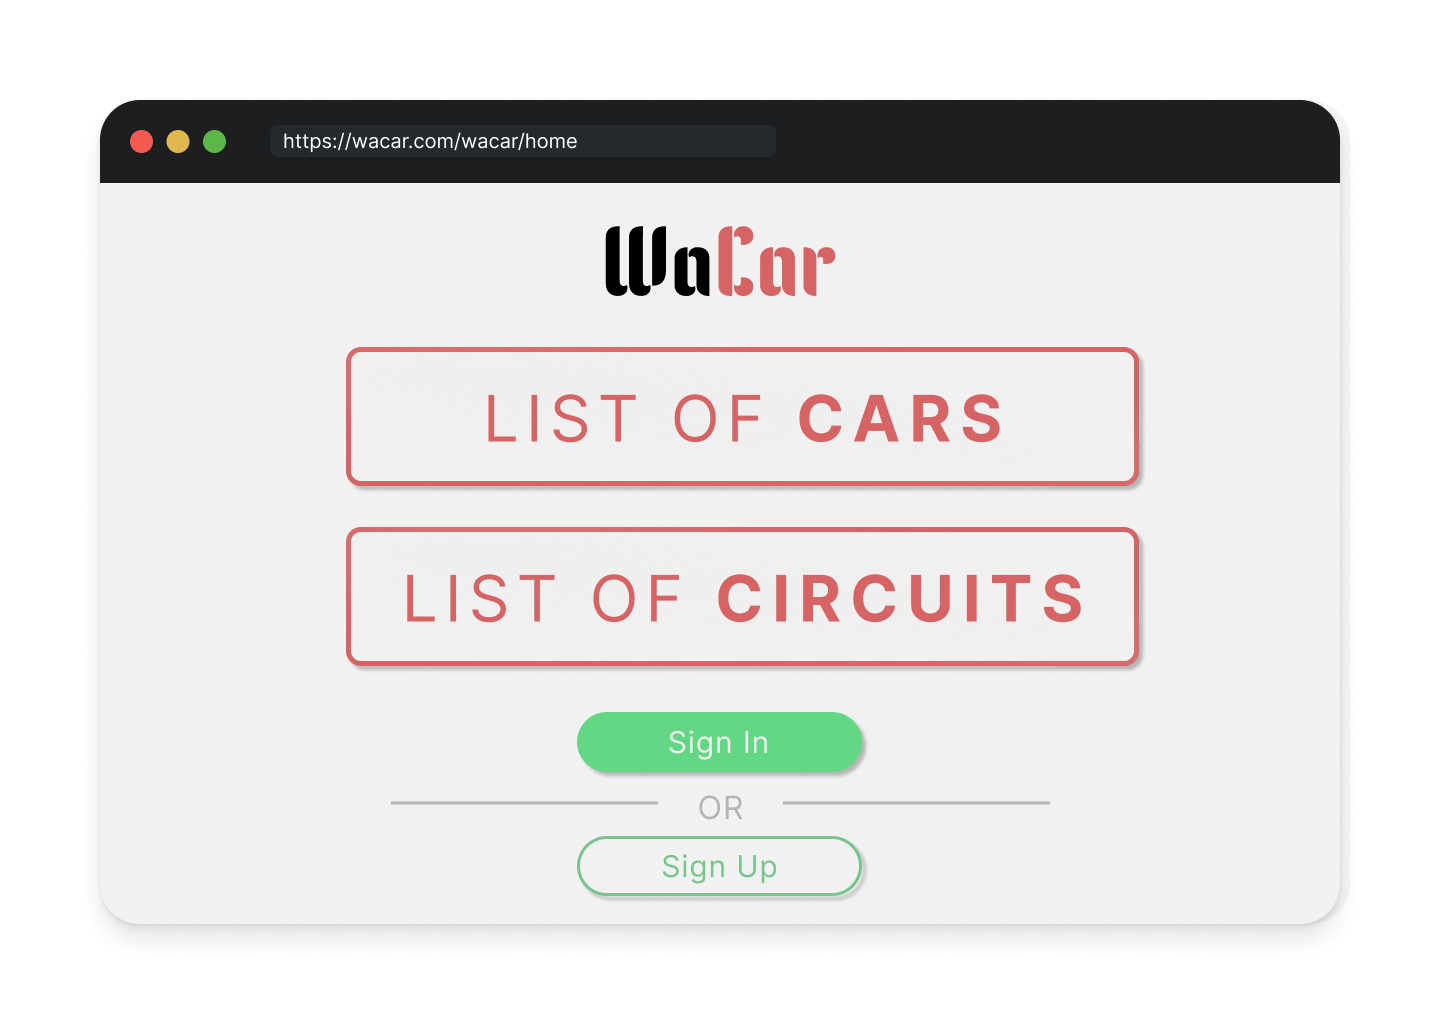
\includegraphics[width=0.6\textwidth]{mockup/NoLogHome.png}
    \caption{Homepage without logging.}
    \label{fig:nologhome}
\end{figure}

\begin{figure}[h]
    \centering
    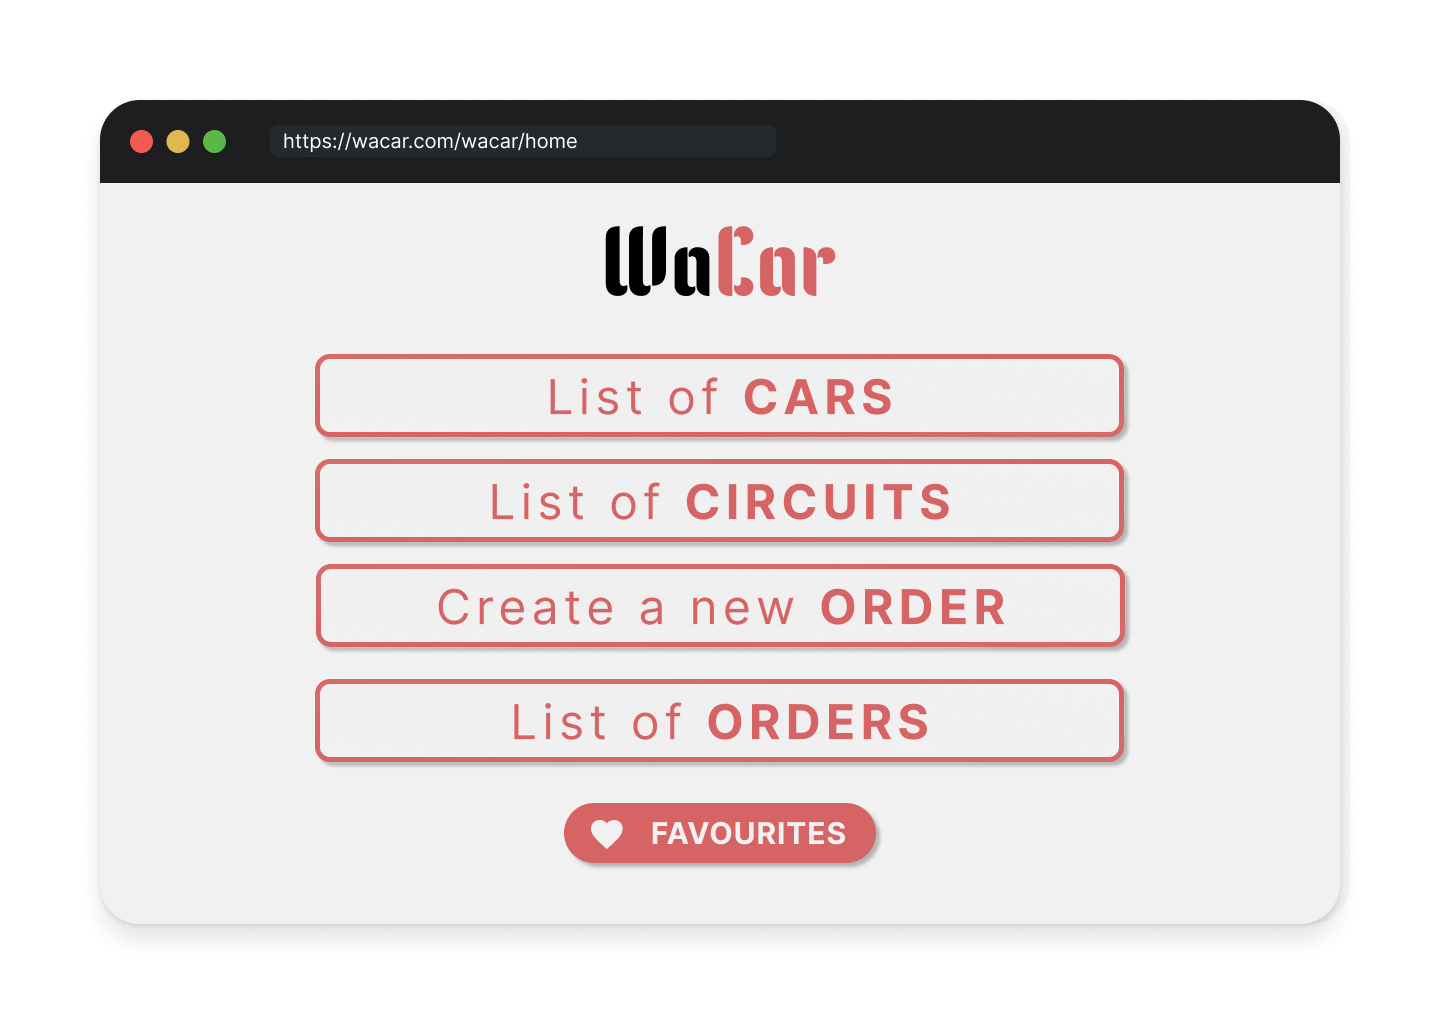
\includegraphics[width=0.6\textwidth]{mockup/UserHome.png}
    \caption{User Homepage.}
    \label{fig:usehome}
\end{figure}

\begin{figure}[h]
    \centering
    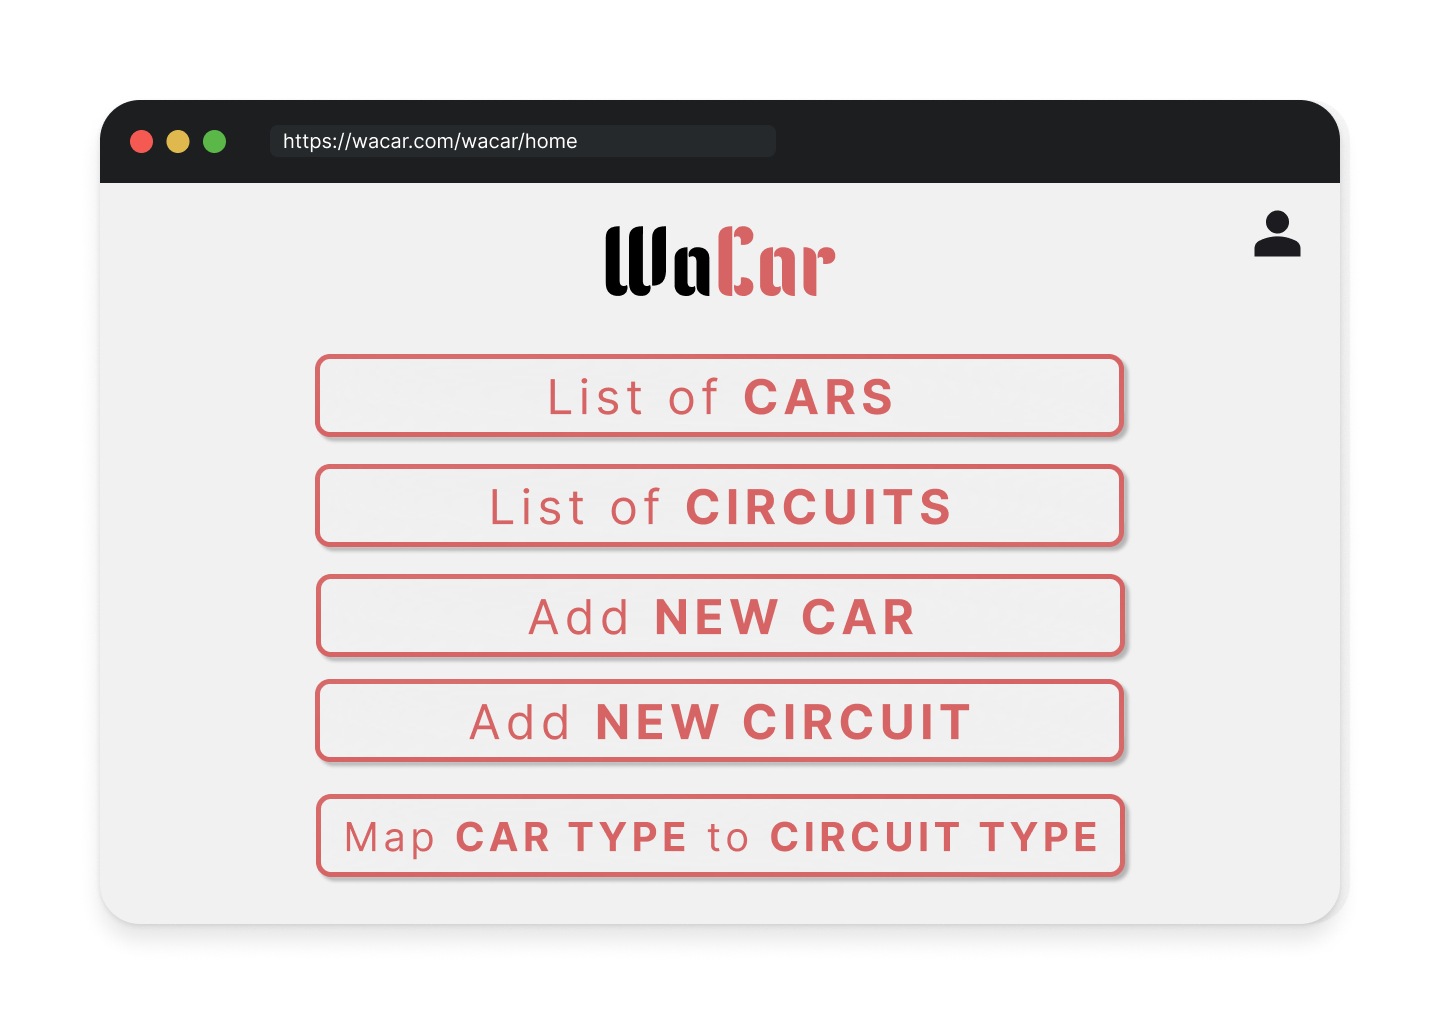
\includegraphics[width=0.6\textwidth]{mockup/AdminHome.png}
    \caption{Admin Homepage.}
    \label{fig:adminhome}
\end{figure}

The homepage serves as the initial landing point for users upon entering WaCar. Its content dynamically adapts to the session state: when user is not logged in, Fig. \ref{fig:nologhome}, they are able to access two basic options that are \texttt{List of Cars} and \texttt{List of Circuits}. Additionally, \texttt{Login} and \texttt{Sign Up} buttons are provided.

If the user is logged in, in addition to the previously mentioned functionalities, \texttt{List of Orders} option and \texttt{Favourite} option are added, Fig. \ref{fig:usehome}. The latter allows the user to manage its favourite objects (car, circuit and even pending orders added to favourite) while through \texttt{List of Orders} the user is able to view his orders history and manage the booked ones.

If an admin is logged in different functionalities are added to its home page as shown in Fig. \ref{fig:adminhome}. The new features are \texttt{Add New Car}, \texttt{Add New Circuit} and \texttt{Map Car Type to Circuit Type} and allows the admin to manage such components according to the possible modification needed.

\subsection{Car list and Circuit list}

\begin{figure}[h]
  \centering
    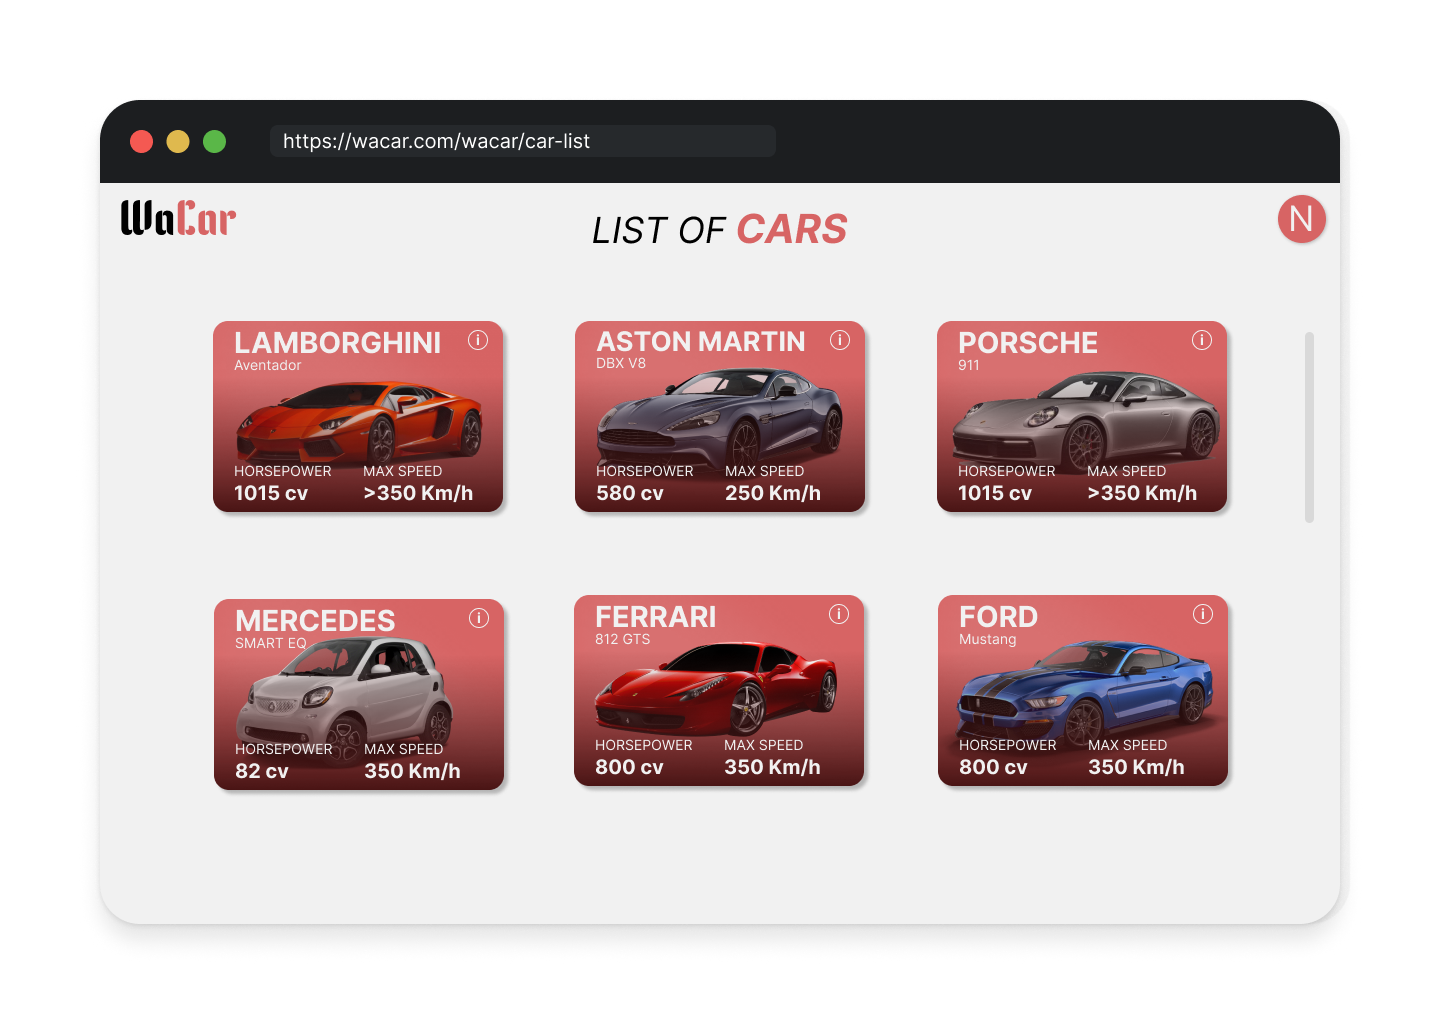
\includegraphics[width=0.6\textwidth]{mockup/CarList.png}
    \caption{Car list page.}
    \label{fig:carlist}
\end{figure}

\begin{figure}[h]
    \centering
    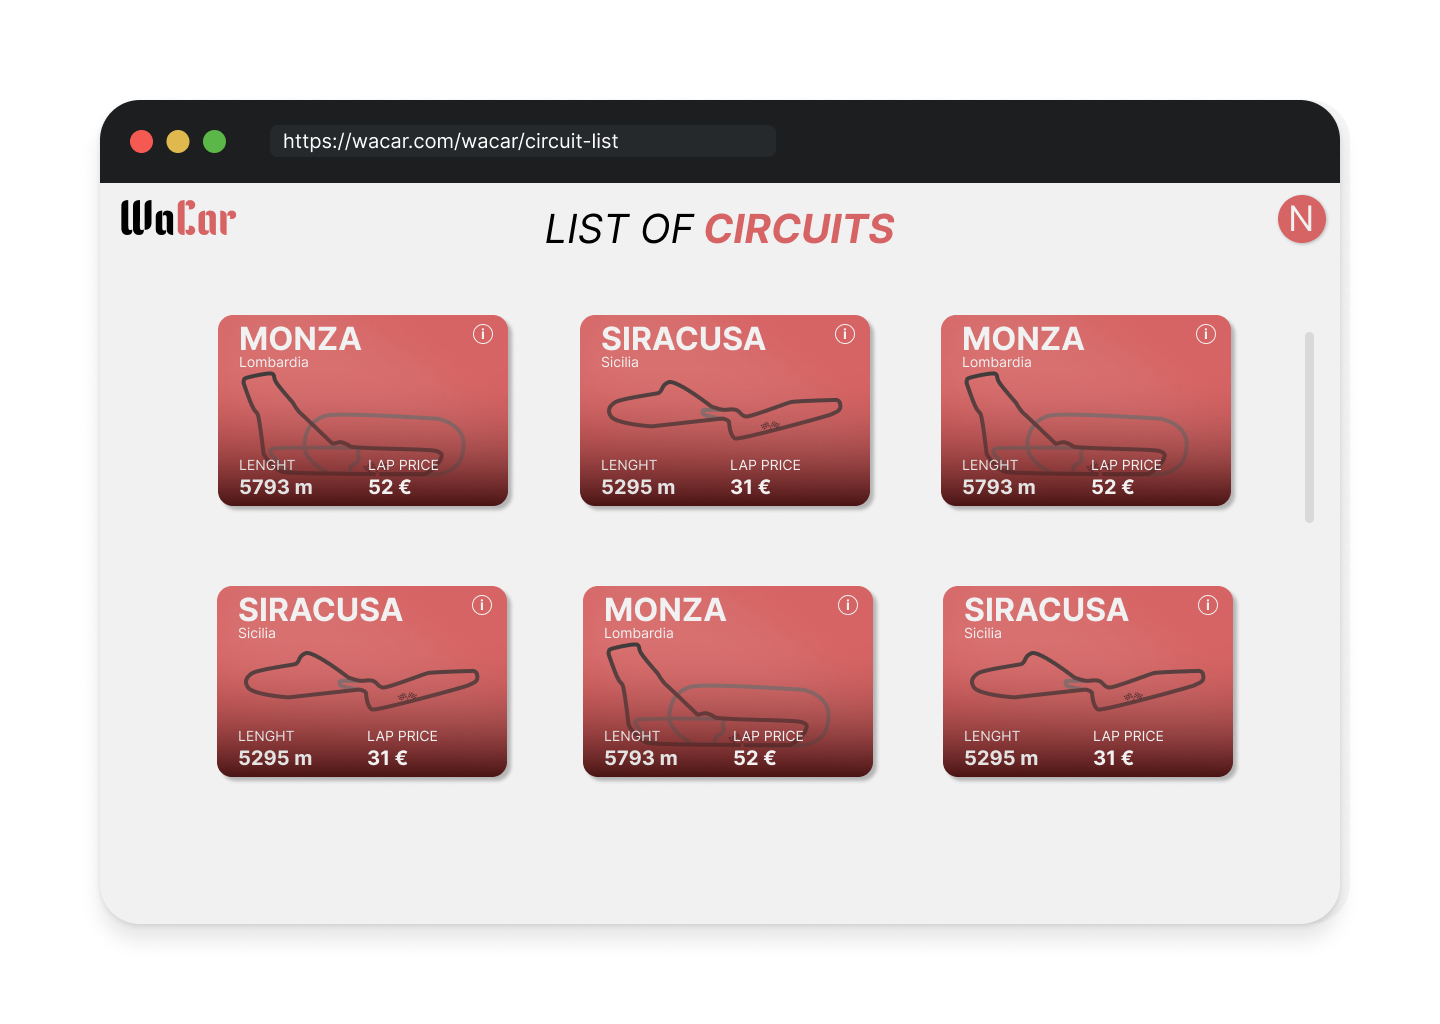
\includegraphics[width=0.6\textwidth]{mockup/CircuitList.png}
    \caption{Circuit list page.}
    \label{fig:circuitlist}
\end{figure}

\begin{figure}[!h]
    \centering
    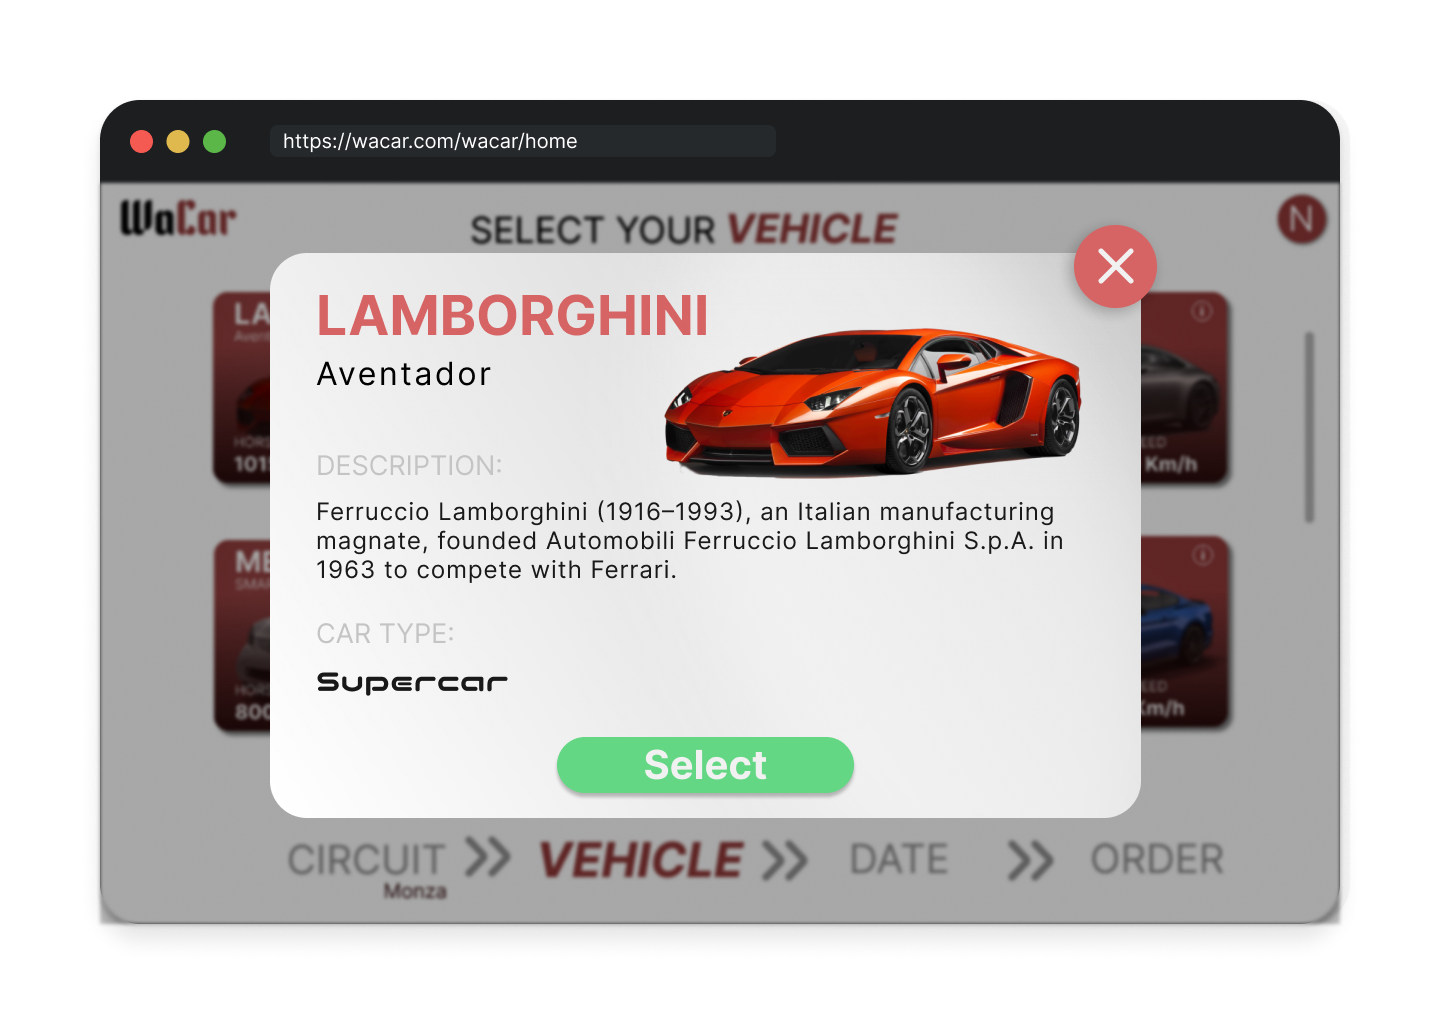
\includegraphics[width=0.6\textwidth]{mockup/InfoCar.png}
    \caption{Car information pop up.}
    \label{fig:infocar}
\end{figure}

Car list, Fig. \ref{fig:carlist}, and Circuit list, Fig. \ref{fig:circuitlist}, pages are two basic pages that allows the user to visualize the possible cars and circuits they can select for their experience. Upon clicking over a car a series of detailed information of the latter are visualized in order to allow the user to better understand the car characteristics as shown in Fig. \ref{fig:infocar}. Analogously, an identical functionality is implemented also in the Circuit list page.

\subsection{Create order and Order recap page}

The create order page displayed in Fig. \ref{fig:allinone} is a one page version for the process of creating an order and a different version may be implemented for the final version of WaCar. The process of creating an order consists in:

\begin{itemize}
    \item selecting a car between the available ones;
    \item selecting an available circuit in which the selected car is suitable to race;
    \item selecting an available date and time for the user experience;
    \item selecting the number of laps that the user is intended to race;
\end{itemize}

After the latter steps the page will display the price for the experience selected by the user and will give the possibility to him/her to print the reservation or if the user decides to not process the order immediately, to save the latter in the favourites and recover it later.

\begin{figure}[h]
    \centering
    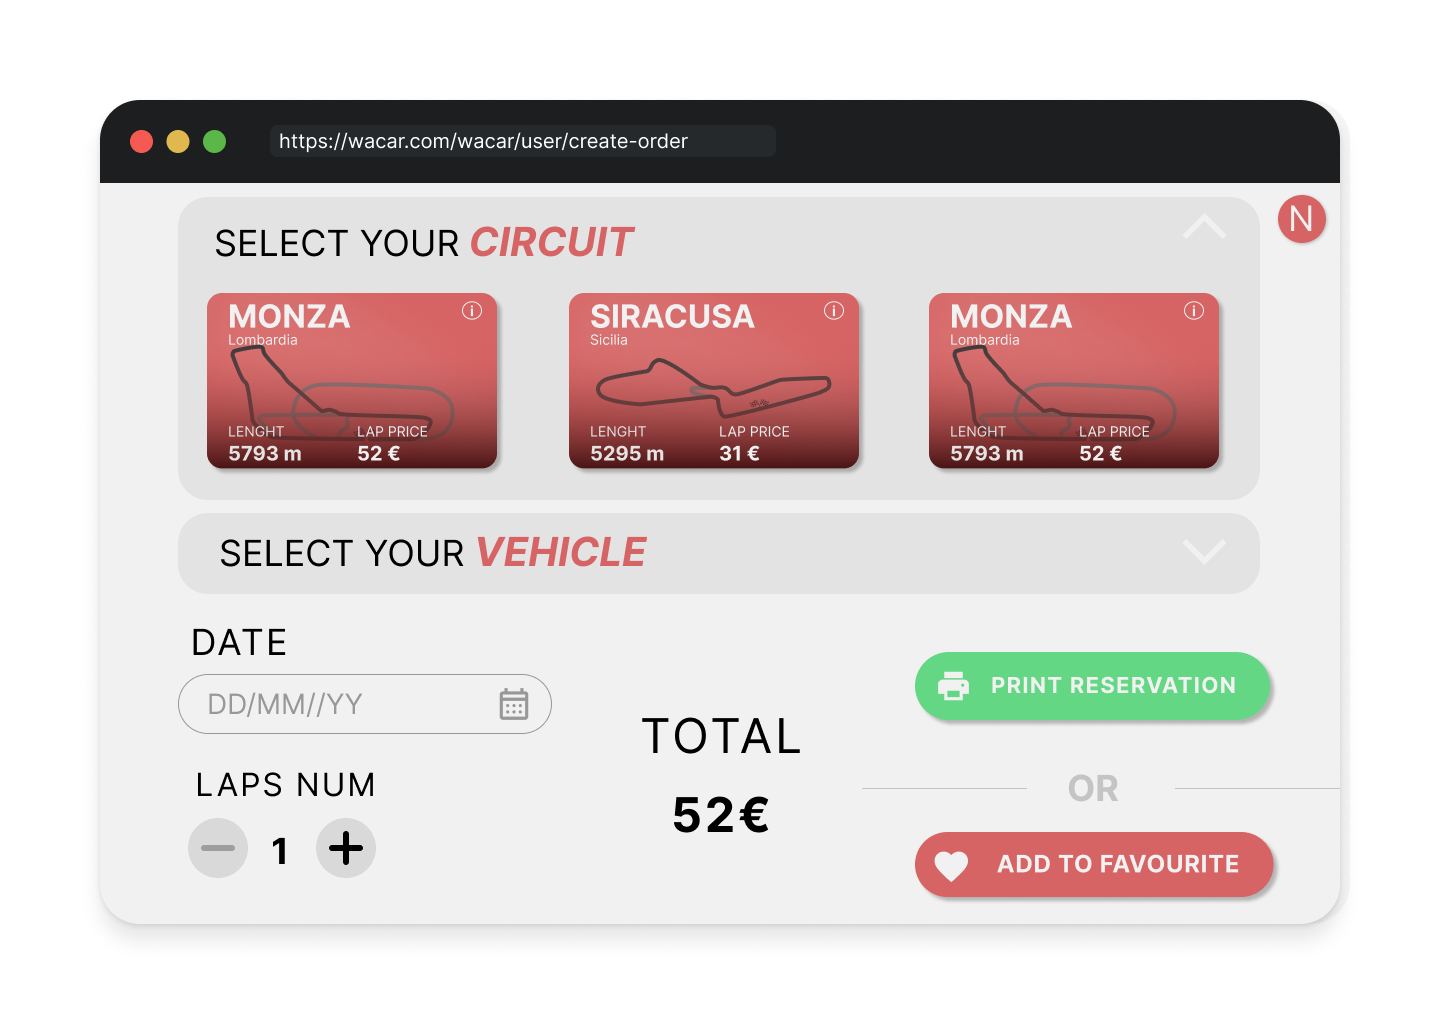
\includegraphics[width=0.6\textwidth]{mockup/OrderAllInOne.png}
    \caption{Order all in one page}
    \label{fig:allinone}
\end{figure}